\documentclass[letterpaper, 12]{article}

%% Language and font encodings
\usepackage[english]{babel}
\usepackage[utf8x]{inputenc}
\usepackage[T1]{fontenc}

%% Sets page size and margins
\usepackage[letterpaper,top=2.5cm,bottom=2cm,left=2cm,right=2cm,marginparwidth=1.75cm]{geometry}

%% Useful packages
\usepackage{amsmath}
\usepackage{amssymb}
\usepackage{amsfonts}
\usepackage{graphicx}
\usepackage{physics}
\usepackage{bbold}
\usepackage[colorinlistoftodos]{todonotes}
\usepackage[colorlinks=true, allcolors=blue]{hyperref}
\usepackage{listings}
\usepackage{multicol}
\usepackage{float}
\usepackage{enumitem}

\usepackage{bm}
\date{\today}

\title{CSC411 Assignment 3}
\author{Yue Guo}
\begin{document}
\maketitle

%%%%%%%%%%%Q1 	20 NEWS GROUP  %%%%%%%%%%%%%%
\section{20 News Group}
\subsection{Top 3 Algorithms}
\subsubsection{Neural Network}
\begin{enumerate}

    \item Hypterparameter: number of layers
	
	In the code nn\_news, I have tried a single layer neural network vs multi-layered neural network.  It turns out that the single neural network is the fastest and also most accurate.

	\item Train/test loss
	\begin{itemize}
     \item  Train accuracy 0.971451299275
     \item Test accuracy 0.632235793946
        \end{itemize}
      \item My expectations
      
      This meets my expectation because NNs are good at working with a large dataset with many feartures. When I increase the number of hidden layers, accuracy decreases. I think this is because it overfits.
  
\end{enumerate}

\subsubsection{Random forest}
\begin{enumerate}

    \item Hypterparameter: number of estimators
	
	I have tried Ensamble with 10 to 150 estimators, and 150 works best after comparing results from cross validation.

	\item Train/test loss
	\begin{itemize}
     \item  Train accuracy 0.974721583878
     \item Test accuracy 0.59346787042
        \end{itemize}
      \item My expectations
      
      This meets my expectations because Random Forest adds more randomness in each step, and ensamble method is more resistant to overfitting because it assigns weights to different features in each step. I also tried decision\_tree, and it does not generalize well.
      The number of estimators learns better with a larger group of weak learners.
  
\end{enumerate}

\subsubsection{SVM - Best Classifier}
\begin{enumerate}

    \item Hypterparameter
	
	In the code, I have tried different rand\_state and cross validated each. It turns out $rand_state = 0$ is the best
	
	\item Train/test loss
	\begin{itemize}
     \item  Train accuracy  0.972511932119
     \item Test accuracy 0.691980881572
        \end{itemize}
        \item Test confusion matrix
        
        The most confused classes are class 10 and 19

\resizebox{\columnwidth}{!}{%
\setcounter{MaxMatrixCols}{20}
$\begin{matrix}
 	0.0 & 70.0 & 75.0 & 73.0 & 66.0 & 76.0 & 71.0 & 77.0 & 79.0 & 78.0 & 80.0 & 77.0 & 74.0 & 77.0 & 75.0 & 79.0 & 45.0 & 57.0 & 9.0 & 68.0 \\
	70.0 & 0.0 & 5.0 & 3.0 & 4.0 & 6.0 & 1.0 & 7.0 & 9.0 & 8.0 & 10.0 & 7.0 & 4.0 & 7.0 & 5.0 & 9.0 & 25.0 & 13.0 & 79.0 & 138.0 \\
	75.0 & 5.0 & 0.0 & 2.0 & 9.0 & 1.0 & 4.0 & 2.0 & 4.0 & 3.0 & 5.0 & 2.0 & 1.0 & 2.0 & 0.0 & 4.0 & 30.0 & 18.0 & 84.0 & 143.0 \\
73.0 & 3.0 & 2.0 & 0.0 & 7.0 & 3.0 & 2.0 & 4.0 & 6.0 & 5.0 & 7.0 & 4.0 & 1.0 & 4.0 & 2.0 & 6.0 & 28.0 & 16.0 & 82.0 & 141.0 \\
66.0 & 4.0 & 9.0 & 7.0 & 0.0 & 10.0 & 5.0 & 11.0 & 13.0 & 12.0 & 14.0 & 11.0 & 8.0 & 11.0 & 9.0 & 13.0 & 21.0 & 9.0 & 75.0 & 134.0 \\
76.0 & 6.0 & 1.0 & 3.0 & 10.0 & 0.0 & 5.0 & 1.0 & 3.0 & 2.0 & 4.0 & 1.0 & 2.0 & 1.0 & 1.0 & 3.0 & 31.0 & 19.0 & 85.0 & 144.0 \\
71.0 & 1.0 & 4.0 & 2.0 & 5.0 & 5.0 & 0.0 & 6.0 & 8.0 & 7.0 & 9.0 & 6.0 & 3.0 & 6.0 & 4.0 & 8.0 & 26.0 & 14.0 & 80.0 & 139.0 \\
77.0 & 7.0 & 2.0 & 4.0 & 11.0 & 1.0 & 6.0 & 0.0 & 2.0 & 1.0 & 3.0 & 0.0 & 3.0 & 0.0 & 2.0 & 2.0 & 32.0 & 20.0 & 86.0 & 145.0 \\
79.0 & 9.0 & 4.0 & 6.0 & 13.0 & 3.0 & 8.0 & 2.0 & 0.0 & 1.0 & 1.0 & 2.0 & 5.0 & 2.0 & 4.0 & 0.0 & 34.0 & 22.0 & 88.0 & 147.0 \\
78.0 & 8.0 & 3.0 & 5.0 & 12.0 & 2.0 & 7.0 & 1.0 & 1.0 & 0.0 & 2.0 & 1.0 & 4.0 & 1.0 & 3.0 & 1.0 & 33.0 & 21.0 & 87.0 & 146.0 \\
80.0 & 10.0 & 5.0 & 7.0 & 14.0 & 4.0 & 9.0 & 3.0 & 1.0 & 2.0 & 0.0 & 3.0 & 6.0 & 3.0 & 5.0 & 1.0 & 35.0 & 23.0 & 89.0 & 148.0 \\
77.0 & 7.0 & 2.0 & 4.0 & 11.0 & 1.0 & 6.0 & 0.0 & 2.0 & 1.0 & 3.0 & 0.0 & 3.0 & 0.0 & 2.0 & 2.0 & 32.0 & 20.0 & 86.0 & 145.0 \\
74.0 & 4.0 & 1.0 & 1.0 & 8.0 & 2.0 & 3.0 & 3.0 & 5.0 & 4.0 & 6.0 & 3.0 & 0.0 & 3.0 & 1.0 & 5.0 & 29.0 & 17.0 & 83.0 & 142.0 \\
77.0 & 7.0 & 2.0 & 4.0 & 11.0 & 1.0 & 6.0 & 0.0 & 2.0 & 1.0 & 3.0 & 0.0 & 3.0 & 0.0 & 2.0 & 2.0 & 32.0 & 20.0 & 86.0 & 145.0 \\
75.0 & 5.0 & 0.0 & 2.0 & 9.0 & 1.0 & 4.0 & 2.0 & 4.0 & 3.0 & 5.0 & 2.0 & 1.0 & 2.0 & 0.0 & 4.0 & 30.0 & 18.0 & 84.0 & 143.0 \\
79.0 & 9.0 & 4.0 & 6.0 & 13.0 & 3.0 & 8.0 & 2.0 & 0.0 & 1.0 & 1.0 & 2.0 & 5.0 & 2.0 & 4.0 & 0.0 & 34.0 & 22.0 & 88.0 & 147.0 \\
45.0 & 25.0 & 30.0 & 28.0 & 21.0 & 31.0 & 26.0 & 32.0 & 34.0 & 33.0 & 35.0 & 32.0 & 29.0 & 32.0 & 30.0 & 34.0 & 0.0 & 12.0 & 54.0 & 113.0 \\
57.0 & 13.0 & 18.0 & 16.0 & 9.0 & 19.0 & 14.0 & 20.0 & 22.0 & 21.0 & 23.0 & 20.0 & 17.0 & 20.0 & 18.0 & 22.0 & 12.0 & 0.0 & 66.0 & 125.0 \\
9.0 & 79.0 & 84.0 & 82.0 & 75.0 & 85.0 & 80.0 & 86.0 & 88.0 & 87.0 & 89.0 & 86.0 & 83.0 & 86.0 & 84.0 & 88.0 & 54.0 & 66.0 & 0.0 & 59.0 \\
68.0 & 138.0 & 143.0 & 141.0 & 134.0 & 144.0 & 139.0 & 145.0 & 147.0 & 146.0 & 148.0 & 145.0 & 142.0 & 145.0 & 143.0 & 147.0 & 113.0 & 125.0 & 59.0 & 0.0 \\  
\end{matrix}%
$}



      \item My expectations
     
      SVM is the best out of all. I think it is because it has a linear decision boundary and does not overfit on training data. The test accuracy is close to single neuron neural net, but still higher.
  
\end{enumerate}

\subsubsection{Bernoulli Baseline}
\begin{enumerate}
	\item Train/test loss
	\begin{itemize}
     \item  Train accuracy  0.598727240587
     \item Test accuracy 0.457912904939
        \end{itemize}
\end{enumerate}





%%%%%%%%%%%Q2 SVM %%%%%%%%%%%%%%
\section{SVM}
\subsection{SVM test}
\begin{figure}[H]
\centering
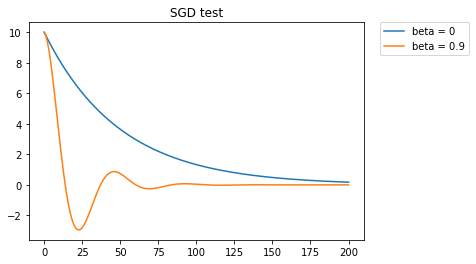
\includegraphics[width=0.5\textwidth]{q2part1plot.png}
\caption{\label{}Plot of test SVM}
\end{figure}

\subsection{SVM code}
see code

\subsection{SVM on MINIST}
\subsubsection{without momentum}
\begin{enumerate}
	\item Train loss$=0.400699029921$
	\item Test loss$=0.37243523202$
	\item classification accuracy on training set $= 0.826985854189$
	\item classification accuracy on testing set $=0.818503401361$
\end{enumerate}

\subsubsection{with momentum}
\begin{enumerate}
	\item classification accuracy on training set $= 0.817555313747$
	\item classification accuracy on testing set $=0.809977324263$
\end{enumerate}

\begin{figure}[H]
\centering
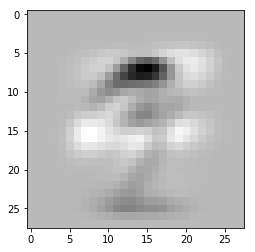
\includegraphics[width=0.5\textwidth]{q2_3_1.png}
\caption{\label{}Plot momentum = 0 }
\end{figure}

\begin{figure}[H]
\centering
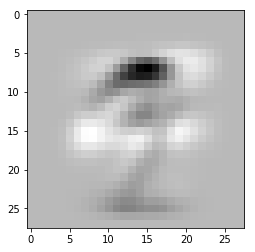
\includegraphics[width=0.5\textwidth]{q_2_3_2.png}
\caption{\label{}Plot momentum = 0.1 }
\end{figure}



%%%%%%%%%%%Q3%%%%%%%%%%%%%%
\section{Kernels}
%%%%%%%%%% q 3.1%%%%%%%%%%%%%%
\subsection{Positive semidefinite and quadratic form}
Assume K is symmetric, we can decompose K into $U \Lambda U^T$
\begin{equation*}
\begin{split}
x^T K x &= x^T (U \Lambda U^T) x = (x^T U) \Lambda (U^T x)\\
\end{split}
\end{equation*}

$\Lambda$ has the eigenvalues $\lambda_{i}$, and if $K$ is positive, and all $\lambda_{i}$ > 0,

\begin{equation*}
\begin{split}
x^T K x &= \Sigma_{i =1}^{d} \lambda_{i} ([x^T U_{i}])^2 >= 0\\
\end{split}
\end{equation*}

Then $x^T K x >= 0$ for all $x$ in $ \mathbb{R}^{d}$ iff $K$ is postive semidefinite

%%%%%%%%%Q 3.2 %%%%%%%%%%%%%%
\subsection{Kernel properties}
%%%%%%%% Q 3.2 q2%%%%%%%%%%%%%
\subsubsection{$\alpha$}
Define mapping $\phi (x) = \sqrt{\alpha}$, $\alpha > 0$, and the kernel $\langle \phi(x), \phi(y) \rangle = \alpha$.
The resulting matrix K has item $K_{ij} = \alpha $, the matrix K has equal number of row and columns, and element is $\alpha$. Since $\alpha$ > 0, and all elements are equal, K is positive semidefinite
 
 %%%%%%%Q 3.2 q3 %%%%%%%%%%%%%%
\subsubsection{$f(x), f(y)$}
$K_{ij} = \langle \phi (x),  \phi (y) \rangle$, \\
define $\phi(x) = f(x), \forall f: \mathbb{R}^{d} \rightarrow \mathbb{R}$\\
define $\phi(y) = f(y), \forall f: \mathbb{R}^{d} \rightarrow \mathbb{R}$\\
Since f(x) and f(y) produce a scalar,  $\langle \phi (x),  \phi (y) \rangle = f(x) \cdot f(y)$

%%%%%%%%Q3.2 part 3%%%%%%%%%%%
\subsubsection{k1 and k2}
If the gram matrix, $K_{1}$ of kernel k1 and gram matrix, $K_{2}$ of kernel k2 are positive semidefinite, by scaling them and adding each element, the new gram matrix of $a \cdot k_{1}(x, y) + b \cdot k_{2}(x, y)$, call it $K$, each element of K is positive since a ,b > 0.\\
$K$ is also symmetric because $K_{1}$ and $K_{2}$ are symmetric with the same dimension, and element wise addition and linear combination preserve the symmetric property.\\

%%%%%%%%Q3.2 part 4%%%%%%%%%%%
\subsubsection{$k(x, y) = \frac{k_{1}(x ,y) }{\sqrt{k_{1}(x, x)} \sqrt{k_{1}(y, y)} }$}
Let $\phi_{1}$ be the mapping defined by $k_{1}$\\
We define a new mapping, $\phi$ for $k(x ,y)$\\
We let $\phi(x) = \frac{\phi_{1} (x)}{\norm{\phi_{1}(x)}}$\\
\begin{equation*}
\begin{split}
k(x, y) &= \langle \phi (x), \phi (y) \rangle \\
&= \frac{\phi_{1}(x)}{\norm{\phi_{1}(x)}} \cdot  \frac{\phi_{1}(y)}{\norm{\phi_{1}(y)}}\\
&= \frac{\phi_{1}(x)}{\sqrt{\phi_{1}(x) \cdot \phi_{1}(x)}} \cdot \frac{\phi_{1}(y)}{\sqrt{\phi_{1}(y) \cdot \phi_{1}(y)}}\\
&= \frac{\phi_{1}(x)}{( \sqrt{\phi_{1}(x)} \cdot \sqrt{ \phi_{1}(y)}  )}  \cdot \frac{\phi_{1}(y)}{( \sqrt{\phi_{1}(x)} \cdot \sqrt{ \phi_{1}(y)}  )} \\
&= \frac{\phi_{1}(x)}{ \sqrt{\phi_{1}(x) \cdot  \phi_{1}(y) }}  \cdot  \frac{\phi_{1}(x)}{ \sqrt{\phi_{1}(x) \cdot  \phi_{1}(y) }}\\
 k(x, y) &= \frac{k_{1}(x ,y) }{\sqrt{k_{1}(x, x)} \sqrt{k_{1}(y, y)} }
\end{split}
\end{equation*}
Therefore, there is a new mapping $\phi(x)$ that supports $k(x, y)$ and it is a kernel because $\phi(x)$
is the product of two kernel mappings

\end{document}